\documentclass[12pt,a4paper,twoside,openright,titlepage,final]{article}
\usepackage{fontspec}
\usepackage{amsmath}
\usepackage{amsfonts}
\usepackage{amssymb}
\usepackage{makeidx}
\usepackage{graphicx}
\usepackage[hidelinks,unicode=true]{hyperref}
\usepackage[spanish,es-nodecimaldot,es-lcroman,es-tabla,es-noshorthands]{babel}
\usepackage[left=3cm,right=2cm, bottom=4cm]{geometry}
\usepackage{natbib}
\usepackage{microtype}
\usepackage{ifdraft}
\usepackage{verbatim}
\usepackage[obeyDraft]{todonotes}
\ifdraft{
	\usepackage{draftwatermark}
	\SetWatermarkText{BORRADOR}
	\SetWatermarkScale{0.7}
	\SetWatermarkColor{red}
}{}
\usepackage{booktabs}
\usepackage{longtable}
\usepackage{calc}
\usepackage{array}
\usepackage{caption}
\usepackage{subfigure}
\usepackage{footnote}
\usepackage{url}
\usepackage{tikz}

\setsansfont[Ligatures=TeX]{texgyreadventor}
\setmainfont[Ligatures=TeX]{texgyrepagella}

%*******************************************************
%                 NO MODIFICAR
\newcommand*{\FSfont}[1]{%
  \fontencoding{T1}\fontfamily{#1}\selectfont}

\newlength{\tpheight}\setlength{\tpheight}{0.9\textheight}
\newlength{\txtheight}\setlength{\txtheight}{0.9\tpheight}
\newlength{\tpwidth}\setlength{\tpwidth}{0.9\textwidth}
\newlength{\txtwidth}\setlength{\txtwidth}{0.9\tpwidth}
\newlength{\drop}
%*******************************************************

% Crea una portada con los siguientes parámetros
%
% #1 : Título 
% #2 : Subtítulo
% #3 : Subsubtítulo
% #4 : Autor(es)
% #5 : Lugar
%

\newcommand*{\portada}[5]{
\begin{titlepage}
\begingroup
\vspace*{1cm}
\drop = 0.2\txtheight
\centering
\vfill
{\Huge \scshape #1}\\[\baselineskip]
{\Large \textbf{#2}}\\[\baselineskip]
{\Large \scshape #3}\\[\baselineskip]
\vspace*{0.3cm}
{\large \textit{#4}}\\[0.5\drop]

\includegraphics[scale=0.35]{./imagenes/logoURJC.jpg}
\vspace*{1.5cm}

{\large \scshape #5, \today} \par
\begin{center}
\end{center}
\vfill\null
\endgroup
\end{titlepage}
}
 %*****************************************************
 


\author{José Ignacio Escribano}

\title{Caso práctico II}

\setlength{\parindent}{0pt}

\begin{document}

\pagenumbering{alph}
\setcounter{page}{1}

\portada{Caso Práctico III}{Modelización y tratamiento de la incertidumbre}{Inferencia}{José Ignacio Escribano}{Móstoles}

\listoffigures
\thispagestyle{empty}
\newpage

\tableofcontents
\thispagestyle{empty}
\newpage


\pagenumbering{arabic}
\setcounter{page}{1}

\section{Introducción}

Este caso práctico consta de dos partes relativas a dos modelos distintos: el primero es acerca del modelo beta-binomial, y el segundo, sobre el modelo normal-normal. En ambas partes se piden calcular intervalos de probabilidad y contrastes de hipótesis, entre otras cosas.

\section{Estimando proporciones y predicción de futuras muestras}

En esta primera parte, consideramos una población de 29 niños que tenían un contenido en plomo en los dientes de leche superior a 22.22 partes por millón, de los cuales, 22 terminaron la Educación Secundaria, y 7 que no lo hicieron. Consideraremos que la distribución a priori de la proporción $p$ de niños que terminaron la Educación Secundaria sigue una distribución $p \sim \mathcal{B}e(1,1)$.\\

Lo primero que tenemos que calcular es la función de verosimilitud $\mathcal{L}(p) = P(X = x | p)$. Sabemos que sólo hay dos resultados posibles: terminar o no terminar la Educación Secundaria, por lo que tenemos una distribución binomial con $n = 29$ y $x = 22$.\\

Por tanto, la función de verosimilitud es:

\begin{align*}
\mathcal{L}(p) & = P(X = 22|p) \\ &= \binom{29}{22} p^{22} (1-p)^{29-22} \\ & \propto p^{22} (1-p)^{29-22} \\ & = p^{22}(1-p)^{7}
\end{align*}

Por otro lado, tenemos como distribución a priori una $\mathcal{B}e(1,1)$. La función de densidad de la distribución $\mathcal{B}e(\alpha, \beta)$ viene dada por

\begin{equation*}
f(p|\alpha, \beta) = \begin{cases}
\dfrac{\Gamma(\alpha + \beta)}{\Gamma(\alpha) + \Gamma(\beta)}p^{\alpha - 1}(1-p)^{\beta - 1}, & \text{si } 0 \leq p \leq 1\\
0, & \text{en otro caso} 
\end{cases}
\end{equation*} 

donde $\Gamma(\cdot)$ denota función gamma definida como

\begin{equation*}
\Gamma(x) = \int_{0}^{\infty} t^{x-1}e^{-t} \, dt
\end{equation*}

Por tanto,

\begin{align*}
f(p | \alpha = 1, \beta = 1) & = \dfrac{\Gamma(1 + 1)}{\Gamma(1) + \Gamma(1)}p^{0}(1-p)^{0} \\ & \propto 1 
\end{align*}

Tenemos una distribución a priori que no nos da ninguna información sobre $p$.\\

La distribución a posteriori $f(p|x)$ viene dada por

\begin{align*}
f(p|x) & \propto f(p) \cdot \mathcal{L}(p) \\ & \propto 1 \cdot p^{22}(1-p)^{7} \\ & = p^{22}(1-p)^{7}
\end{align*}

Comparando con la definición de función de densidad de una distribución beta, tenemos que la distribución a posteriori $p|x \sim \mathcal{B}e(23,8)$.\\

La Figura~\ref{fig:distribuciones_beta} muestra las distribuciones a priori, a posteriori y la distribución empírica. Ésta última se ha generado generando con 1000 muestras de una distribución $\mathcal{B}e(23,8)$ (nuestra distribución a posteriori) con el comando \texttt{rbeta} de R. Tanto la distribución a posteriori como la distribución empírica son bastante parecidas, por lo que el comando \texttt{rbeta} de R aproxima bien la función aún cunado el número de muestras es relativamente pequeño.\\

\begin{figure}[tbph!]
\centering
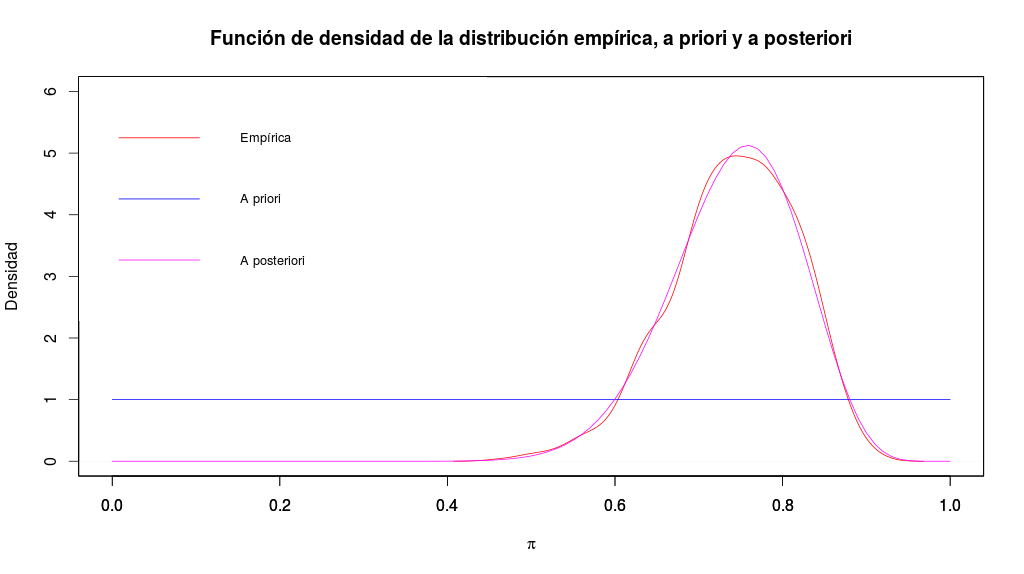
\includegraphics[width=0.9\linewidth]{./imagenes/distribuciones_beta}
\caption{Función de densidad de la distribución empírica, a priori y a posteriori}
\label{fig:distribuciones_beta}
\end{figure}

Como tenemos nuestra distribución a posteriori, podemos calcular la media y la varianza a posteriori de esta distribución, ya que las fórmulas para la media y la varianza son conocidas:

\begin{align*}
E(x|p) & = \dfrac{\alpha}{\alpha + \beta}\\
Var(x|p) & = \dfrac{\alpha \beta}{(\alpha + \beta)^2 (\alpha + \beta + 1)}
\end{align*}

Sustituyendo en las fórmulas anteriores $\alpha$ por 23 y $\beta$ por 8, se tiene que

\begin{align*}
E(x|p) & = 0.7419 \\
Var(x|p) & = 0.0059 \\
s(x|p) & = \sqrt{Var(x|p)} = 0.0773 
\end{align*}

Para calcular el intervalo de probabilidad al 90\% calculamos los cuantiles que acumulan el 5 \% y el 95 \% de nuestra distribución a posteriori. Para ello aplicamos el comando \texttt{qbeta} de R. Así se tiene que el intervalo de probabilidad al 90 \% es $[0.6060, 0.8598]$. La Figura~\ref{fig:intervalo_probabilidad_beta} muestra el intervalo de probabilidad sobre la distribución a posteriori. 

\begin{figure}[tbph!]
\centering
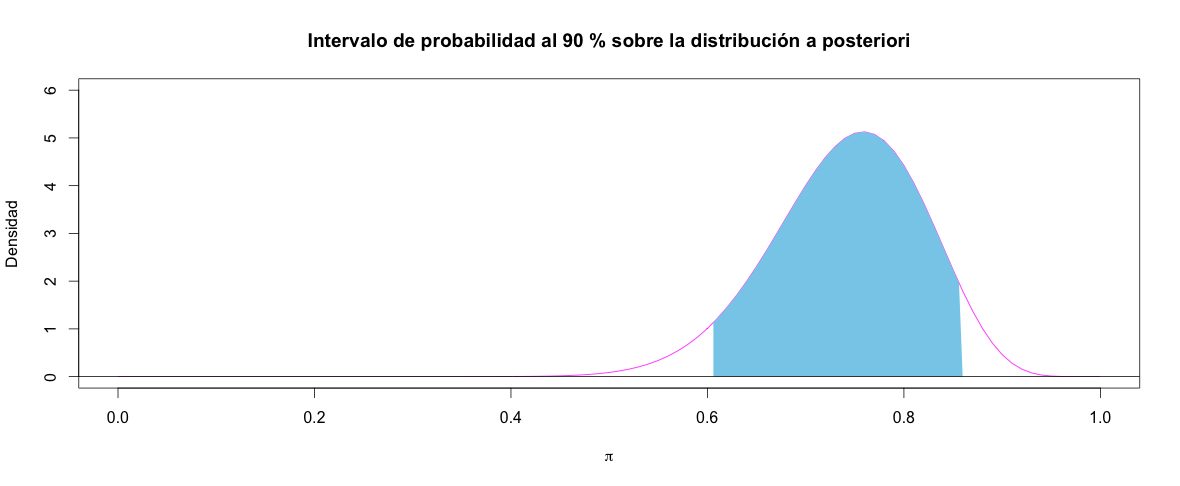
\includegraphics[width=0.9\linewidth]{./imagenes/intervalo_probabilidad_beta}
\caption{Intervalo de probabilidad al 90\% sobre la distribución a posteriori}
\label{fig:intervalo_probabilidad_beta}
\end{figure}

También necesitamos hacer el siguiente contraste de hipótesis:

\begin{align*}
H_0 & : p \leq 0.4 \\
H_1 & : p > 0.4
\end{align*}

Para ello, calculamos la probabilidad de que nuestra distribución a posteriori sea menor que 0.4 y mayor que 0.4. Aplicamos el comando \texttt{pbeta} de R. Así tenemos que

\begin{align*}
P(H_0) & = 4.9325 \cdot 10^{-5} \\
P(H_1) & = 0.9999
\end{align*}

Como $P(H_1) > P(H_0)$, rechazamos la hipótesis nula.\\

Por último, vamos a calcular la probabilidad predictiva del modelo beta-binomial de que haya $k$ éxitos en los $m$ siguientes ensayos, que viene dada por

\begin{equation*}
P(k \text{ éxitos en } m | x) = \binom{m}{k} \dfrac{\Gamma(\alpha + \beta + n)}{\Gamma(\alpha + x) \Gamma(\beta + n - x)} \dfrac{\Gamma(\alpha + x + k) \Gamma(\beta + n - x + m - k)}{\Gamma(\alpha + \beta + m + n)}
\end{equation*}

donde $\Gamma(\cdot)$ es la función gamma definida como anteriormente, $\alpha$ y $\beta$ son los parámetros de nuestra distribución beta a priori, $x$ es el número de éxitos y $n$ es el número de éxitos.\\

En nuestro caso, tenemos que $\alpha = \beta = 1$, $x = 22$ y $n = 29$. Hay que calcular la probabilidad de que al menos 9 de los 10 próximos niños terminen la Educación Secundaria.\\

Si denotamos con $H$ al número de niños que terminan la Educación Secundaria entre 10 posibles, entonces

\begin{align*}
P(H \geq 9 | x) & = 1 - P(H < 9 | x) \\ & = 1 - P(H \leq 8 | x) \\ & = 1 - \sum_{k=0}^{8} P(k \text{ niños acaban la Educación Secundaria de } 10 | x) \\ & = 1 - (0.00031 + 0.00209 + 0.00931 + 0.03026 + 0.07542 + 0.14666 \\ & + 0.22095 + 0.24857 + 0.19026) \\ & = 1 - 0.92389 \\ & = 0.07610
\end{align*}

Por tanto, la probabilidad predictiva de que al menos 9 de los 10 próximos niños acaben la Educación Secundaria es del 7.61 \%.\\

La función de densidad de la probabilidad predictiva se muestra en la Figura~\ref{fig:distribucion_predictiva_beta}.

\begin{figure}[tbph!]
\centering
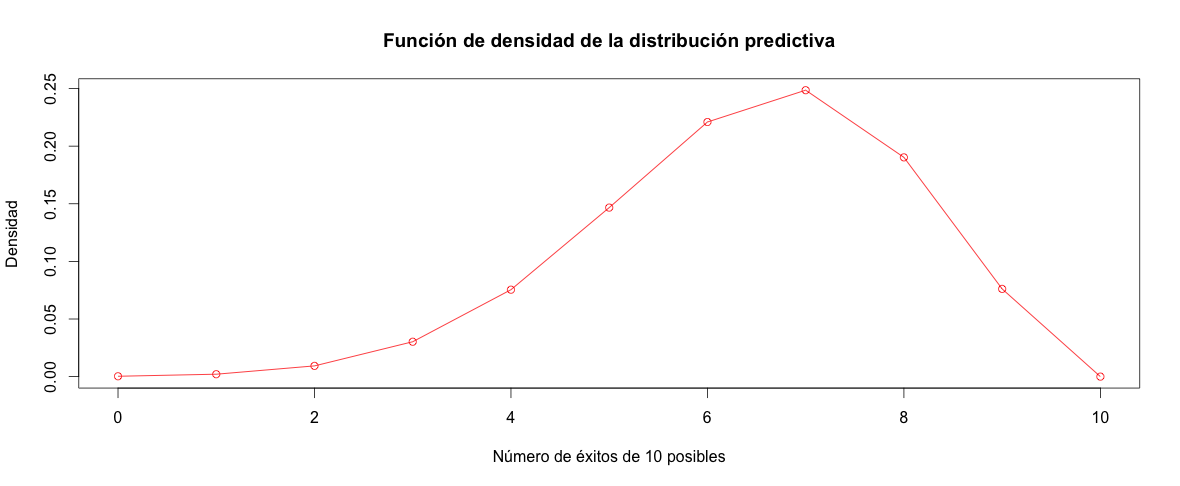
\includegraphics[width=0.9\linewidth]{./imagenes/distribucion_predictiva_beta}
\caption{Función de densidad de la distribución predictiva}
\label{fig:distribucion_predictiva_beta}
\end{figure}

\section{Estimando una media normal con una a priori discreta}

En esta segunda parte, queremos estimar la precipitaciones totales en forma de nieve. Los datos recogidos $y_i$ provienen de una distribución normal con media $\mu$ y desviación típica $\sigma = 10$.

La distribución a priori viene dada por la siguiente función de densidad:

\begin{equation*}
f(\mu) = \begin{cases}
0.1, & \text{si } \mu = 20 \\
0.15, & \text{si } \mu = 30 \\ 
0.25, & \text{si } \mu = 40 \\
0.25, & \text{si } \mu = 50 \\ 
0.15, & \text{si } \mu = 60 \\
0.1, & \text{si } \mu = 70
\end{cases}
\end{equation*}

La Figura~\ref{fig:distribucion_priori_normal} muestra esta distribución.

\begin{figure}[tbph!]
\centering
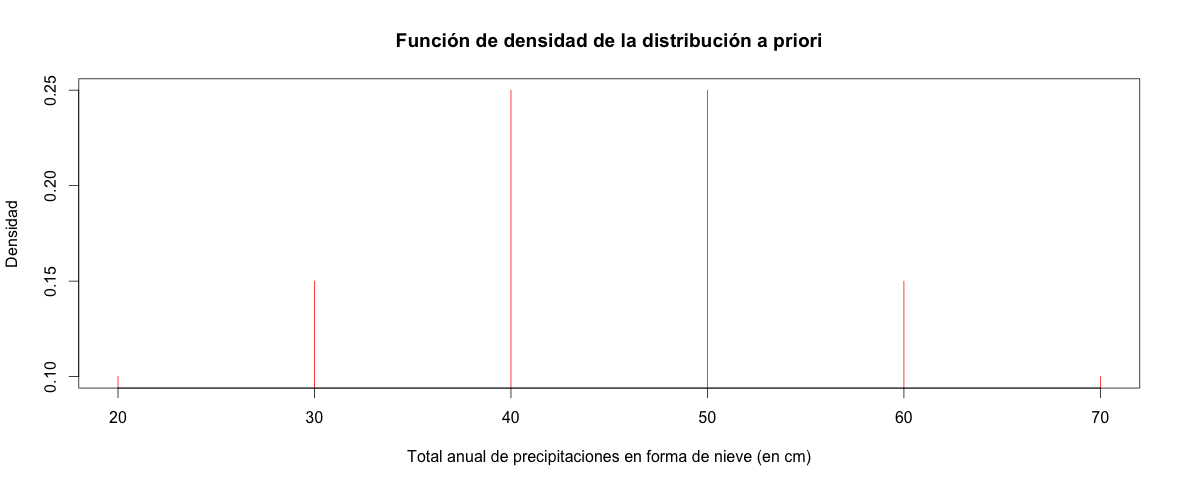
\includegraphics[width=0.9\linewidth]{./imagenes/distribucion_priori_normal}
\caption{Función de densidad de la distribución a priori}
\label{fig:distribucion_priori_normal}
\end{figure}

La función de verosimilitud para este modelo viene dada por

\begin{align*}
\mathcal{L}(\mu) & = \left(\dfrac{1}{\sqrt{2\pi} \sigma}\right)^n \prod_{i=1}^{n} \exp \left[ -\dfrac{1}{2} \left( \dfrac{y_i - \mu}{\sigma} \right)^2 \right] \\
& = \left(\dfrac{1}{\sqrt{2\pi} \sigma}\right)^n \exp \left[ \sum_{i=1}^{n} -\dfrac{1}{2} \left( \dfrac{y_i - \mu}{\sigma} \right)^2 \right] \\
& = \left(\dfrac{1}{\sqrt{2\pi} \sigma}\right)^n \exp \left[ -\dfrac{1}{2\sigma^2} \sum_{i=1}^{n} \left( y_i^2 + \mu^2 - 2y_i\mu \right) \right] \\
& = \left(\dfrac{1}{\sqrt{2\pi} \sigma}\right)^n \exp \left[ -\dfrac{1}{2\sigma^2} \left( n\mu^2 + \sum_{i=1}^{n} y_i^2 - 2\mu \sum_{i=1}^{n} y_i \right) \right]
\end{align*}

Los valores de $y$ (precipitaciones de nieve en cm) son los siguientes:

\begin{table}[htbp!]
\centering
\resizebox{\textwidth}{!}{%
\begin{tabular}{@{}lllllllllllll@{}}
\toprule
$y$ & $38.6$ & $42.4$ & $57.5$ & $40.5$ & $51.7$ & $67.1$ & $33.4$ & $60.9$ & $64.1$ & $40.1$ & $40.7$ &  \\ \bottomrule
\end{tabular}
}
\end{table}


Calculamos la función de verosimililud para cada uno de los valores de $\mu$ de la distribución a priori.

\begin{table}[htbp!]
\centering
\resizebox{\textwidth}{!}{%
\begin{tabular}{@{}lllllll@{}}
\toprule
\multicolumn{1}{c}{$\mu$} & \multicolumn{1}{c}{$20$} & \multicolumn{1}{c}{$30$} & \multicolumn{1}{c}{$40$} & \multicolumn{1}{c}{$50$} & \multicolumn{1}{c}{$60$} & \multicolumn{1}{c}{$70$} \\ \midrule
$\mathcal{L}(\mu)$ & $8.907 \cdot 10^{-41}$ & $3.315 \cdot 10^{-30}$ & $7.580 \cdot 10^{-25}$ & $1.064 \cdot 10^{-24}$ & $9.193 \cdot 10^{-30}$ & $4.875 \cdot 10^{-40}$ \\ \bottomrule
\end{tabular}
}
\end{table}

Calculamos la distribución a posteriori para $\mu$ como $f(\mu | y) = \mathcal{L}(y|\mu)f(\mu)$.\\

\begin{table}[htbp!]
\centering
\resizebox{\textwidth}{!}{%
\begin{tabular}{@{}ccccccc@{}}
\toprule
$\mathcal{L}(\mu)$ & $8.907 \cdot 10^{-41}$ & $3.315 \cdot 10^{-30}$ & $7.580 \cdot 10^{-25}$ & $1.064 \cdot 10^{-24}$ & $9.193 \cdot 10^{-30}$ & $4.875 \cdot 10^{-40}$ \\ \midrule
$f(\mu)$ & $0.10$ & $0.15$ & $0.25$ & $0.25$ & $0.15$ & $0.10$ \\ \midrule
$f(\mu | y)$ & $9.807 \cdot 10^{-42}$ & $4.972 \cdot 10^{-31}$ & $1.895 \cdot 10^{-25}$ & $2.662 \cdot 10^{-25}$ & $1.378 \cdot 10^{-30}$ & $4.875 \cdot 10^{-41}$ \\ \bottomrule
\end{tabular}
}
\end{table}

Si nos fijamos en los valores de $f(\mu | y)$ vemos que no tenemos una verdadera distribución, puesto que los valores calculados no suman 1. Para que sea una distribución, sumamos todos los valores calculados y dividimos cada valor por la suma mencionada anteriormente.\\

La suma de todos los valores es $4.557 \cdot 10^{-25}$, por lo que debemos dividir entre este valor cada uno de los $f(\mu | y)$. Por tanto, la distribución a posteriori (Figura~\ref{fig:distribucion_posteriori_normal}) es la siguiente:

\begin{table}[htbp!]
\centering
\resizebox{\textwidth}{!}{%
\begin{tabular}{@{}ccccccc@{}}
\toprule
$\mu$ & $20$ & $30$ & $40$ & $50$ & $60$ & $70$ \\ \midrule
$f(\mu | y)$ & $1.954 \cdot 10^{-17}$ & $1.091 \cdot 10^{-6}$ & $4.158 \cdot 10^{-1}$ & $5.841 \cdot 10^{-1}$ & $3.025 \cdot 10^{-6}$ & $1.069 \cdot 10^{-16}$ \\ \bottomrule
\end{tabular}
}
\end{table}

\begin{figure}[tbph!]
\centering
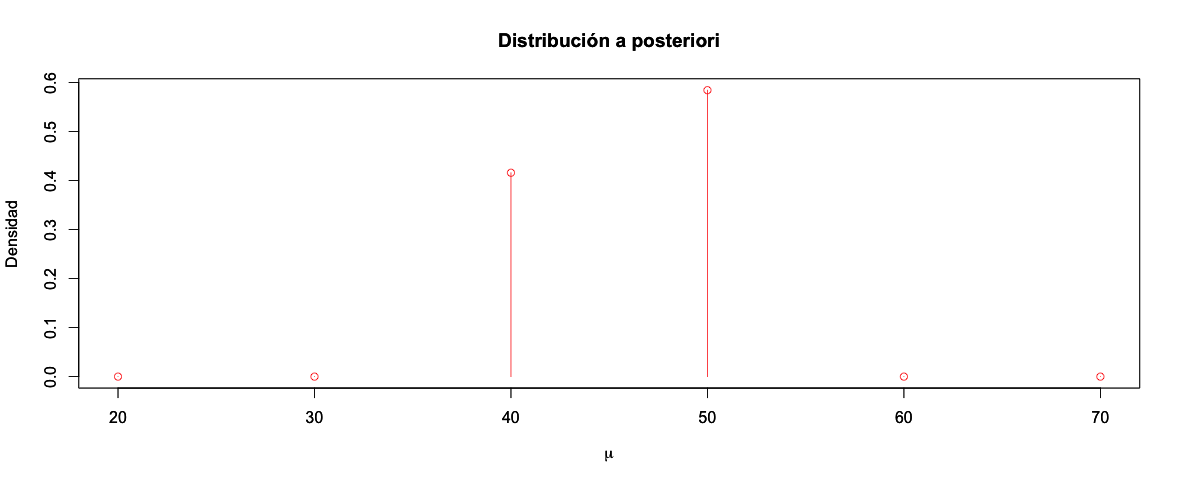
\includegraphics[width=0.9\linewidth]{./imagenes/distribucion_posteriori_normal}
\caption{Función de densidad de la distribución a posteriori}
\label{fig:distribucion_posteriori_normal}
\end{figure}

Si queremos calcular un intervalo de probabilidad al 80 \% para $\mu$, usamos el comando \texttt{discint} de R. Esta función nos devuelve que el intervalo es $[40, 50]$, aunque la probabilidad de este intervalo es del 99.99\%, mayor que el pedido.\\

Si ahora consideramos que la distribución para $\mu \sim \mathcal{N}(\mu_0 = 60, \sigma_0 = 5)$, la distribución a posteriori viene dada por

\begin{align*}
f(\mu | y) & \propto f(\mu) \mathcal{L}(\mu) \\ & \propto \exp \left[ -\dfrac{1}{2} \left( \dfrac{\mu - \mu_0}{\sigma_0} \right)^2  \right] \left\{ \prod_{i=1}^{n} \exp \left[ -\dfrac{1}{2} \left( \dfrac{y_i - \mu}{\sigma} \right) \right] \right\} \\ 
& \propto \exp \left\{ -\dfrac{1}{2} \left( \dfrac{1}{\sigma_0^2} + \dfrac{n}{\sigma^2} \right) \left[ \mu - \left( \dfrac{\dfrac{\mu_0}{\sigma_0^2} + \dfrac{n \bar{y}}{\sigma^2}}{\dfrac{1}{\sigma_0^2} + \dfrac{n}{\sigma^2}} \right)\right]^2 \right\}
\end{align*}

Por tanto, $p|y \sim \mathcal{N}\left(\dfrac{\dfrac{\mu_0}{\sigma_0^2} + \dfrac{n \bar{y}}{\sigma^2}}{\dfrac{1}{\sigma_0^2} + \dfrac{n}{\sigma^2}}, \sqrt{\left( \dfrac{1}{\sigma_0^2} + \dfrac{n}{\sigma^2} \right)^{-1}}\right)$.\\

Sustitiyendo, en la formula anterior se tiene que $p|y \sim \mathcal{N}(48.9625, 2.5)$. La Figura~\ref{} muestra las funciones de densidad de las distribuciones a priori y a posteriori.\\

\begin{figure}[tbph!]
\centering
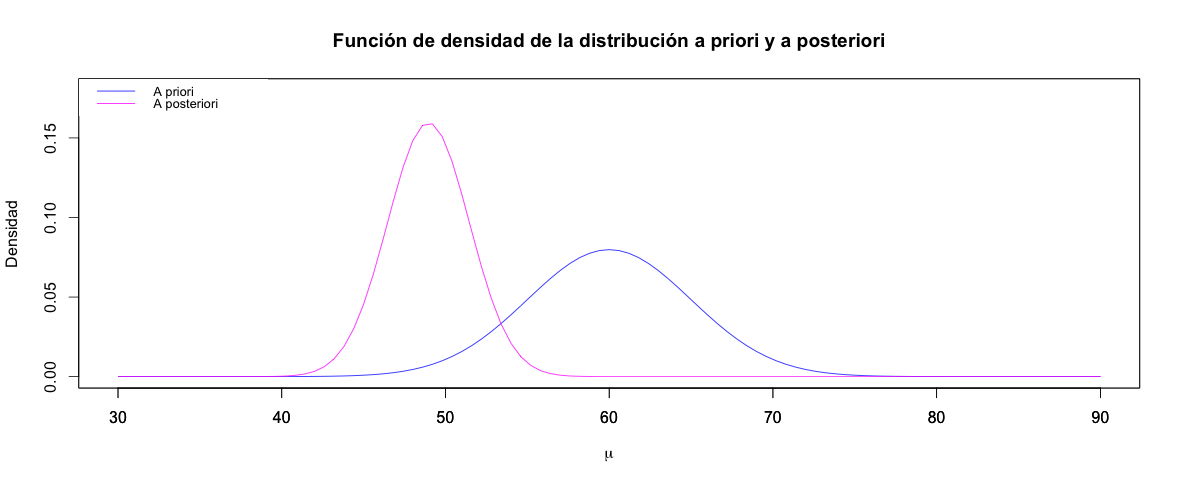
\includegraphics[width=0.9\linewidth]{./imagenes/distribucion_posteriori_normal_normal}
\caption{Función de densidad de la distribución a priori y a posteriori}
\label{fig:distribucion_posteriori_normal_normal}
\end{figure}

Para calcular el intervalo de probabilidad al 80\% para $\mu$ usamos el comando \texttt{qnorm} de R. Usamos los cuantiles 0.1 y 0.9 para obtener el intervalo pedido. R nos devuelve que el intervalo es $[44.850, 53.074]$. En la Figura~\ref{fig:intervalo_probabilidad_normal} se muestra el intervalo de probabilidad al 80\% junto con la distribución a posteriori.

\begin{figure}[tbph!]
\centering
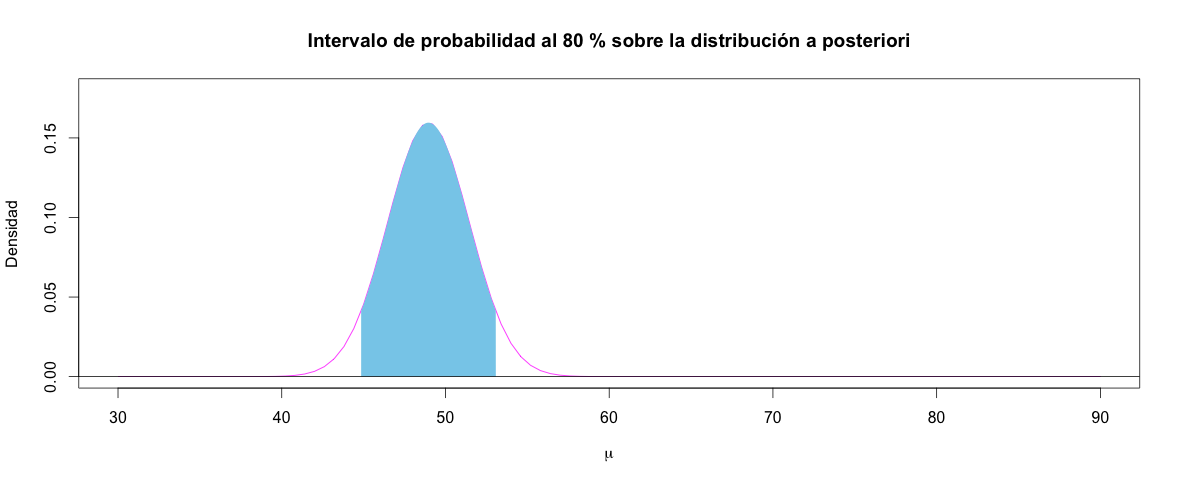
\includegraphics[width=0.9\linewidth]{./imagenes/intervalo_probabilidad_normal}
\caption{Intervalo de probabilidad al 80\% sobre la distribución a posteriori}
\label{fig:intervalo_probabilidad_normal}
\end{figure}

\section{Conclusiones}

En este caso práctico hemos visto dos modelos clásicos de inferencia bayesiana: el modelo beta-binomial y el modelo normal-normal. Hemos puesto en práctica toda la teoría de ambos modelos para calcular probabilidades sobre la distribución a posteriori, intervalos de probabilidad, contrastes de hipótesis, etc. Para calcular todo lo anterior nos hemos del poderoso software estadístico R, que nos ha ahorrado mucho tiempo evitando realizar cálculos tediosos manualmente. 

\newpage

\section{Código R}

\verbatiminput{../caso_iii.R}


\end{document} 